%%%%%%%%%%%%%%%%%%%% author.tex %%%%%%%%%%%%%%%%%%%%%%%%%%%%%%%%%%%
%
%%%%%%%%%%%%%%%% Springer %%%%%%%%%%%%%%%%%%%%%%%%%%%%%%%%%%

\newfloat{Query}{tbp}{lop}

\title*{Using Graph Databases to Explore Genetic Programming Run Dynamics}
% Use \titlerunning{Short Title} for an abbreviated version of
% your contribution title if the original one is too long
\author{Nicholas Freitag McPhee, David Donatucci, and Thomas Helmuth and others(?)}
% Use \authorrunning{Short Title} for an abbreviated version of
% your contribution title if the original one is too long
\institute{Nicholas Freitag McPhee \at University of Minnesota, Morris
\and David Donatucci \at University of Minnesota, Morris
\and Thomas Helmuth \at University of Massachusetts Amherst}

\maketitle

\abstract{Each chapter should be preceded by an abstract (10--15 lines long) that summarizes the content. The abstract will appear \textit{online} at \url{www.SpringerLink.com} and be available with unrestricted access. This allows unregistered users to read the abstract as a teaser for the complete chapter. As a general rule the abstracts will not appear in the printed version of your book unless it is the style of your particular book or that of the series to which your book belongs.}

\begin{keywords}
keywords to your chapter, these words should also be indexed
\end{keywords}
\index{keywords to your chapter}
\index{these words should also be indexed}
\\

\section{Introduction}
\label{sec:introduction}

It is common practice in most empirical evolutionary computation (EC) 
research\marginpar{It would be nice to scrape, say, the GECCO 2014 proceedings and get some 
	numbers to back this up.} to perform numerous (possibly hundreds) of runs, and then simply 
report a handful of aggregate statistics at the end that are expected to summarize and represent 
the (hopefully) complex interactions and dynamics of those many runs. Tables present values such 
as mean or median best fitnesses at the end of runs, collapsing the complexities of dozens or 
hundreds of runs into a single number, possibly with a standard deviation or (even better) a 
confidence interval to give a sense of the distribution. Often more informative are plots, which can, 
for example, show how these numbers change over time during the runs, possibly giving a sense of 
the system dynamics. These plots, however, often aggregate runs in a way that obscure important 
moments that, if explored, might reveal valuable insight into the evolutionary dynamics being 
reported.\marginpar{Perhaps include a sample plot and show how it hides things? One of Tom's 
	diversity or cluster plots? A synthetic plot? Maybe that's just not necessary?}

While this sort of aggregate reporting is often valuable, allowing for important comparative
analysis of, for example, the impact of different genetic operators, it typically fails to provide
any sense of the \emph{why}. Yes, Treatment A led to better aggregate performance than 
Treatment B -- but what happened in the runs that led to that result? Any success at the end of a
run is ultimately the intricate combination of hundreds or thousands of selections, recombinations
and mutations, and if Treatment A is in some sense ``better'' than Treatment B, it must ultimately
be because it affected all those genealogical and genetic events in some significant way, biasing them
towards events that made success more likely. 

Unfortunately, published research very rarely includes information that might shed light on 
these \emph{why} events. We rarely see evolved programs, for example, or any kind of post-run analysis
of those programs, and there is almost never any data or discussion of the genealogical history that
might help us understand how a successful program actually came to be. 

Sometimes this isn't included
for reasons of space and time; evolved programs, for example, are often extremely large and complex,
and a meaningful presentation and discussion of such a program could easily take up more space than
authors have available given the typical space limitations in published work.
Our suspicion, however, is that this sort of \emph{why} analysis often isn't reported because it isn't 
even \emph{done}, in no small part because it's hard. As EC researchers we're in the
``happy'' position of being able to collect anything and everything that happens in a run, but that 
leaves us with two problems: How to \emph{store} the data, and how to \emph{analyze} the data
after it's stored. Decreasing data storage costs have done much to mitigate the first problem.
If, however, one collects a very rich data set it's still easy to quickly generate terabytes of data,
and even if one has a place to put the data, one still needs reasonable tools to analyze the data.

Databases provide a natural tool for storing and accessing the data, but traditional relational
databases are poorly suited for a variety of queries that are important for the genealogical analysis
we need for exploring the evolutionary dynamics of our EC runs. If, for example, we have a 
\texttt{ParentChild} table, it's easy enough to find Alice's parents, but finding Alice's grandparents,
siblings, or cousins requires multiple joins. Moving further out in Alice's tree of relatives
requires complex and computationally expensive recursive joins, making this approach increasingly
infeasible. In exploring the dynamics of an EC run, for example, we're going to want to be able to
make connections across dozens or even hundreds of generations, which simply isn't feasible with a
relational database. (See, for example, \cite{Robinson:GraphDB:Book} for more on these 
feasability/efficiency issues.)

In this chapter we illustrate the use of graph databases as an alternative storage and analysis tool for
evolutionary computation runs. In \cite{donatuccianalysis} we have demonstrated that graph databases
can be an effective tool for analyzing complex genetic programming (GP) dynamics, which led directly
to a proposed change to standard sub-tree crossover in tree-based GP, \cite{mcphee:GECCO15}.
Here we will use the open source Neo4J graph database tool\footnote{\url{http://neo4j.com/}} 
to explore data from a
collection of PushGP runs on several problems drawn from a benchmark collection of introductory 
programming problems taken from \cite{helmuth:GECCO15}.

\section{A little background on problems and tools}

\subsection{Neo4J and Cypher}

Give an example or three of Cypher.

\subsection{PushGP and lexicase selection}

Say a little about
\begin{itemize}
	\item Plush genomes
	\item Push programs
	\item Alternation
	\item The two kinds of mutation
\end{itemize}

Say enough about lexicase so people have some sense of why it might be interesting and different
from, e.g., tournament selection.

\subsection{Replace-space-with-newline}

Say enough about this problem so that people can understand the error vectors.

\section{Lexicase, meet Replace-space-with-newline}

We did one hundred runs of the replace-space-with-newline problem using lexicase selection, and
found that 55 of these succeeded in the sense that an individual was discovered that had zero
error on all 200 of the training cases. Tournament selection with tournament size 7 only
had 13 successes out of 100 runs, and IFS only had 17 successes out of 100 runs, so it seems that
lexicase selection provides a significant advantage here.

\subsection{Hey, we won! But \emph{why}?}

% This is run 6, lexicase, replace-space-with-newline.

It's interesting the lexicase did so well, but that leaves us with the crucial question of \emph{why}? 
So we chose one successful run to explore in more detail. It's important to note
here that we're making no claims that this is a ``representative'' run (whatever that would even
mean); it's an \emph{interesting} run, though, and our hope is that by understanding its dynamics
better we can learn useful things about both the problem and the tools we're applying.

\begin{sidewaysfigure}
	\vspace{0.6\columnwidth}
	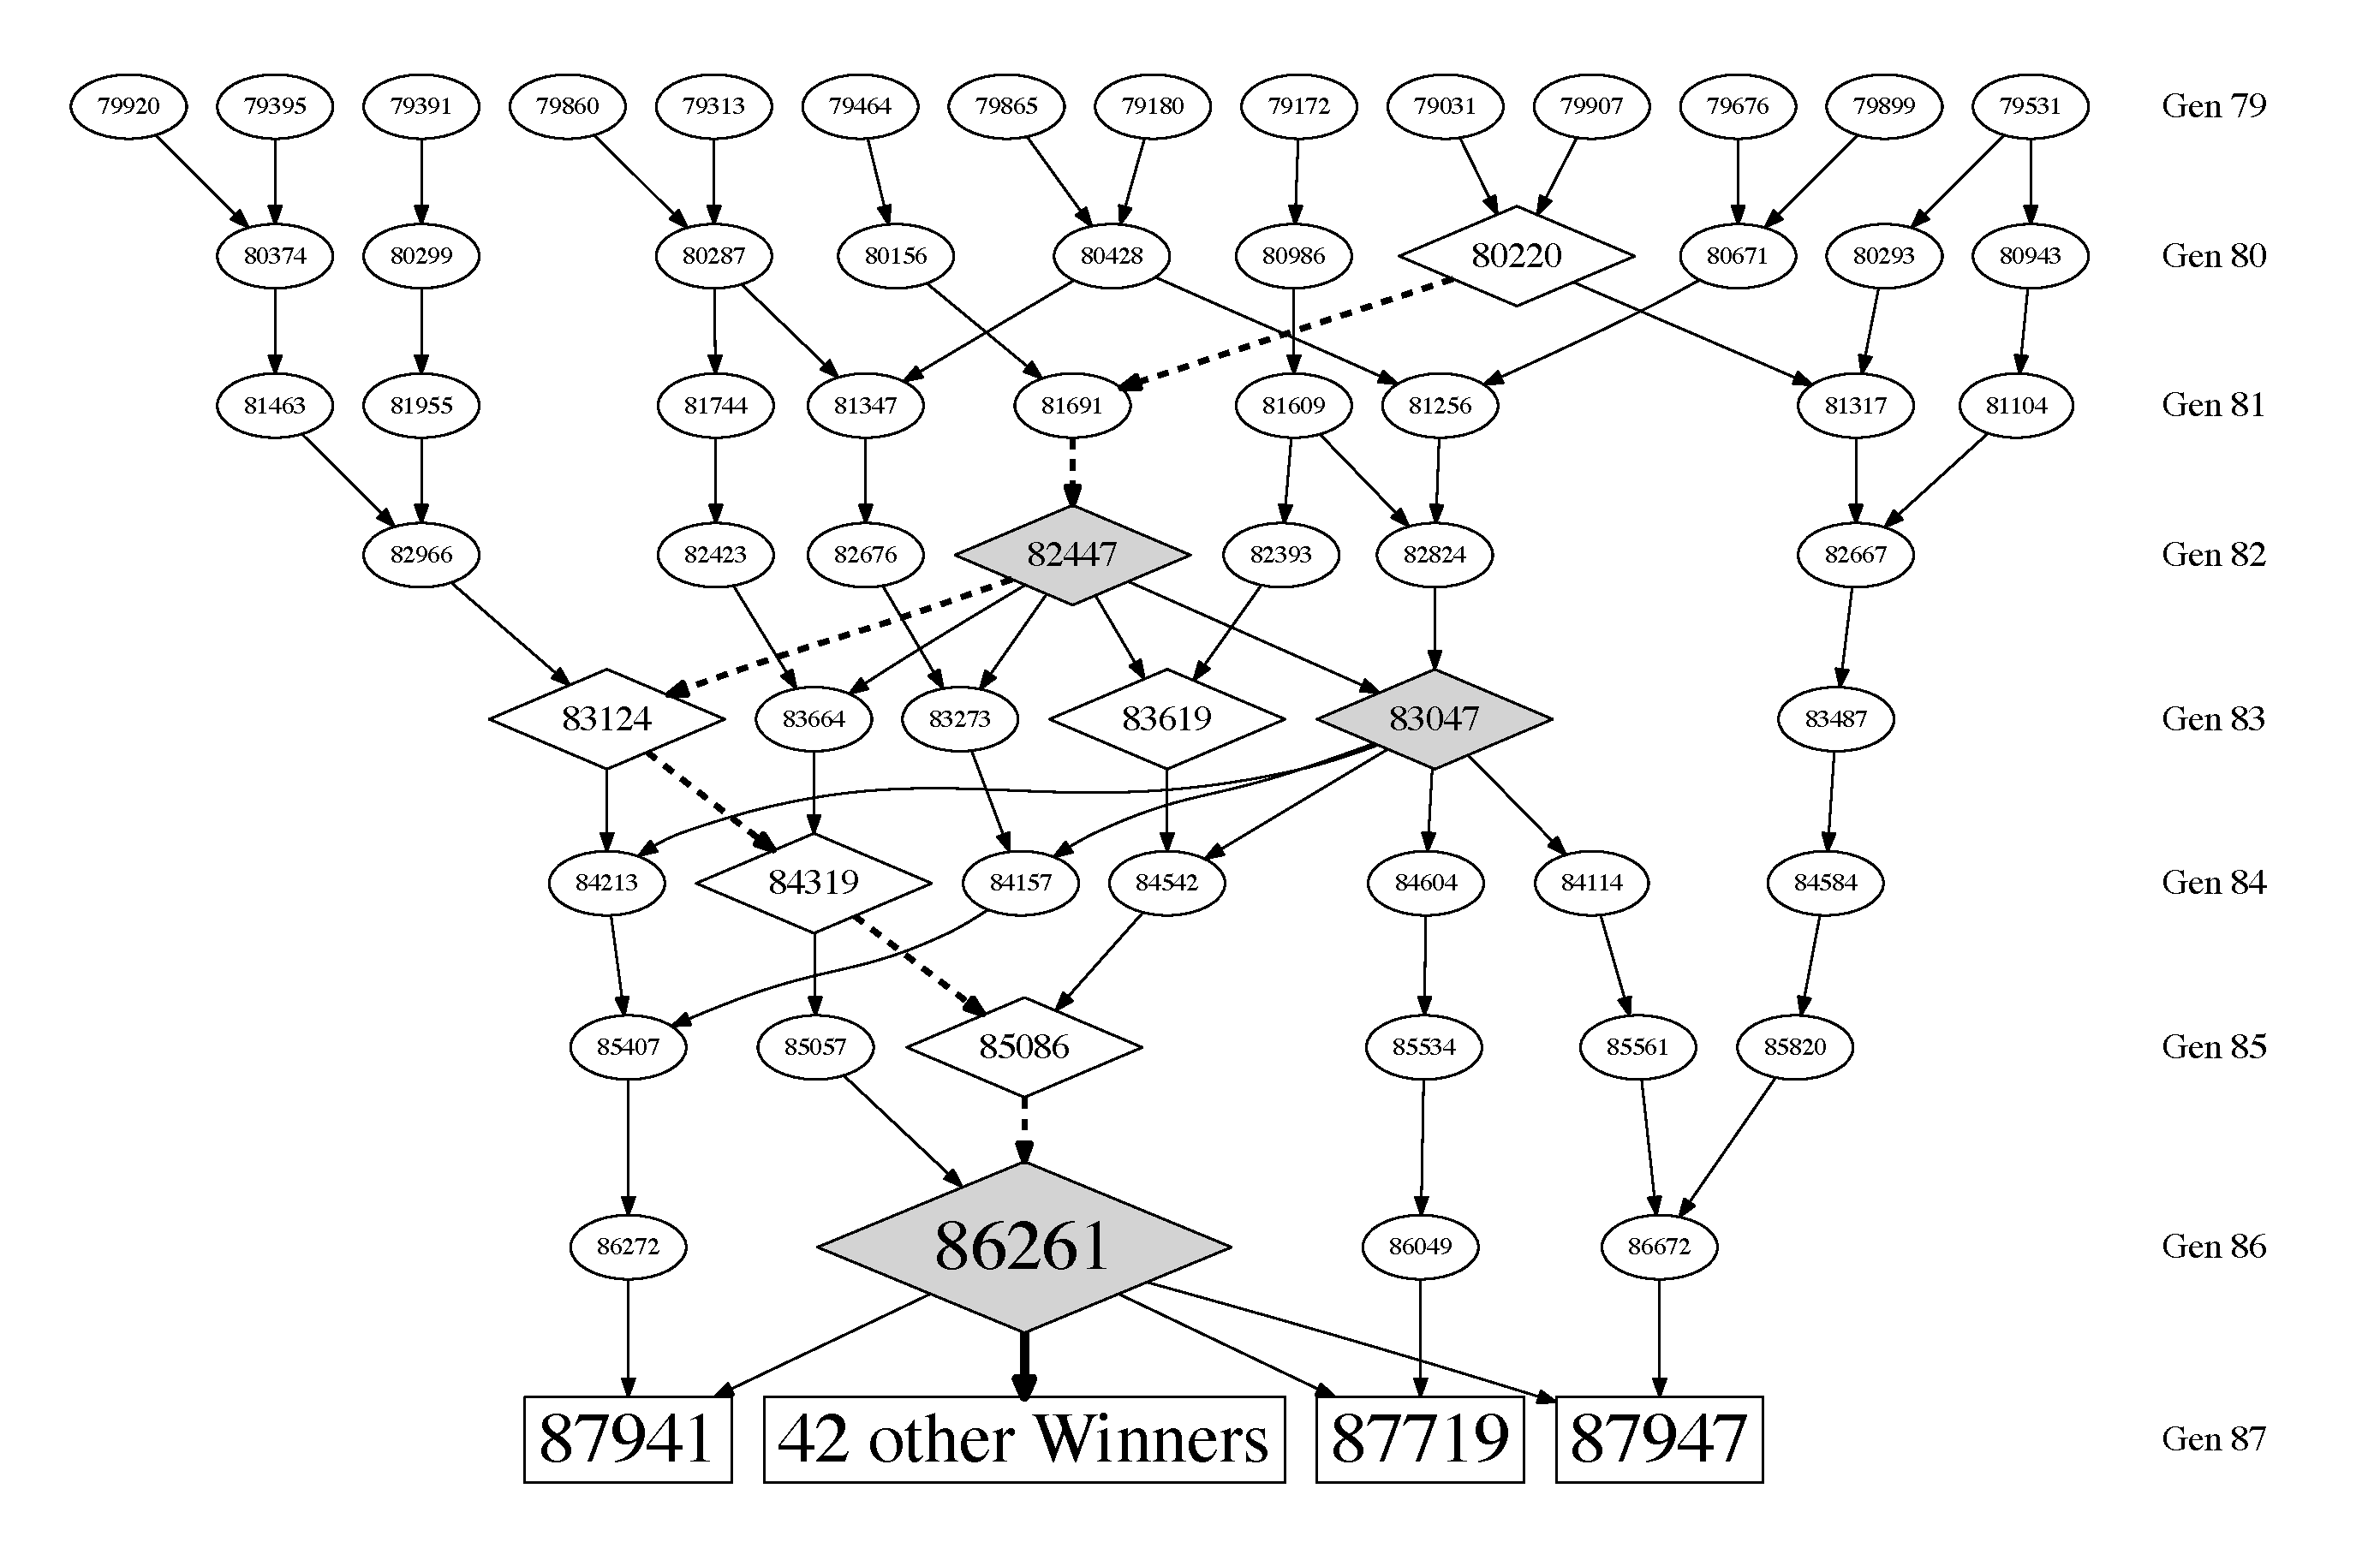
\includegraphics[width=0.88\columnwidth]{figures/ancestors_of_winners.pdf}
	\caption{Ancestry of the 45 ``winners'' from run 6 of lexicase, replace-space-with-newline. Nodes
		with diamonds instead of ellipses had an unusually large number of offspring. Shaded nodes
		had an unusual number of offspring that were ancestors of winners. The dashed lines highlight
		individuals that had an unusually large number of distinct ancestry paths down to a winner.
		See the text for more details}
	\label{fig:winnerAncestors}
\end{sidewaysfigure}

An obvious place to start is at the end when the GP system solved the problem. So we used Neo4J
to find all the ancestors of any ``winning'' individual, i.e., individual with a total error of 
on all 200 test cases. Using Cypher (Neo4J's query language), we can easily ask for this subset
of the population going back to generation 79 using the query in 
Query~\ref{query:winnerAncestors}.\footnote{We could certainly 
	have gone back farther in time, but the graph would have become impossible to read as the
	number of nodes would have ballooned from a few dozen to hundreds or thousands. We went
	back to generation 79 because that was the most recent generation that had more than 10
	distinct ancestors of a winning individual.}\marginpar{Should all the query details go in
	an appendix that eventually becomes a tech report or some such? I'm not sure if they aren't
	just a distraction here.}\marginpar{We need the crazy \texttt{p->c->w} thing in 
	Query~\ref{query:numChildren} to extract 
	single edges, but I don't know if we want to talk about that.}

\begin{Query}
	\begin{verbatim}
	MATCH (p)-->(c)-[*0..7]->(w {total_error: 0}) 
	RETURN DISTINCT id(p), id(c);
	\end{verbatim}
	\caption{Cypher query to find all the ancestors of ``winners'' in the last 9 generations of a run.
		The pattern \texttt{(w \{total\_error: 0\})} matches nodes with total error 0, i.e., 
		``winners''. The pattern \texttt{(c)-[*0..7]->(w)} matches any path from some node \texttt{c} to
		a winning node \texttt{w} that has between 0 and 7 edges.
		}
	\label{query:winnerAncestors}
\end{Query}

Figure~\ref{fig:winnerAncestors} shows the ancestry of all of the winners from generation 87 
(when we first found a winner in this run) back to generation 79.
Each node in the graph represents an individual, and each directed edge indicates a parent-child
relationship, with the edge going from the parent to the child. The numbers inside the nodes are
Neo4J internal IDs; we'll use these as ``names'' for the individuals as we tell the stories we uncover.
\footnote{We actually assign each individual a UUID so we can combine multiple runs, but
	the Neo4J IDs are shorter and easier to use in our story telling.} As a happy accident coming
from having a population size of 1,000, the first two digits of the Neo4J idea also happens to indicate
what generation that individual was from.

Ignoring for the moment the adornments (shape, shading, etc.), there are several things that
we can observe right away:
\begin{itemize}
	\item There are 45 distinct winners in the final generation, or 4.5\% of the population of
	1,000 individual. This tells us that constructing a winner from the individuals in generation 86
	wasn't entirely trivial, but it also wasn't a huge challenge and happened multiple times.
	\item Those 45 winners only had four distinct ancestors in the preceding generation.
	\item All 45 winners had a single individual (86261, marked with a large shaded diamond near
	the center bottom) as at least one of their parents, and 42 of
	them had 86261 as their \emph{only} parent, i.e., they were mutations of 86261, or were the result
	of self-crosses of 86261. To simplify the graph, we've combined those 42 individuals into a
	single node labelled ``42 Winners''.
	\item The number of ancestors of winners doesn't grow quickly as we move back in time. We have to
	go back to generation 80 to find 10 individuals (or 1\% of the population) that are ancestors of
	winners, and in generation 79 there are still only 14 ancestors of winners. In fact we have to
	go back all the way to generation 63 to find a time where over 100 individuals (or over 10\% of 
	the population) were ancestors of a winning individual.
\end{itemize}

Looking at Figure~\ref{fig:winnerAncestors} we can also see that a few individuals have more offspring
represented than others. As we've already mentioned, individual 86261 has 45 successful offspring,
and both individuals 82447 and 83047 have five offspring in the graph, i.e., five offspring that were
ancestors of a winning individual in generation 87. Each of these is marked in 
Figure~\ref{fig:winnerAncestors} with a shaded diamond. 

Figure~\ref{fig:winnerAncestors},
however, only tells us home many offspring an individual had that were themselves either a winner
or an ancestor of a winner, as no other nodes are displayed. 
might, however, wonder how many total offspring an individual has
regardless of whether they were a winner or not. Query~\ref{query:numChildren} identifies the most
fecund ancestors of winners in these last nine generations. That reveals several results that were
quite surprising to at least some of the authors, the most remarkable being that individual 86261 
was a parent of 934 of the 1,000 individiuals in generation 87! Given that lexicase selection was
designed in significant part of spread selection events out across the population, this makes it
clear that there are times when lexicase does the opposite, and instead puts nearly all its eggs in
a single basket. This level of selection focus would simply be impossible using almost any other
common type of selection such as tournament selection; in most uses of tournament selection, 
for example, no individual can be in more than a relative handful of tournaments, and thus can't be
a parent terribly often no matter how fit they are.

While no other node in Figure~\ref{fig:winnerAncestors} has nearly as many children as 86261 did,
there are several that had very high reproduction rates, putting them well above what would be 
possible with something like tournament selection. Individual 82447, for example, had
443 offspring, including the 5 illustrated in Figure~\ref{fig:winnerAncestors}. In fact there were
eight individuals in Figure~\ref{fig:winnerAncestors} that have more than 100 offspring; each of
these is indicated with a diamond shape instead of the standard ellipse. This highlights a particularly
interesting ancestry chain from 82447 through 83124, 84319, 85086 to 86261, each of which had more
than 100 offspring. Here the test case results for each of these individuals must be quite
``special'' in the sense that they are be able to solve an large set of test cases that other
individuals simply aren't able to solve.

\emph{The dashed lines indicate individuals with lots of different paths to a winner, i.e., they
	are the ancestor of a winner in several different ways. we still need to write that up.}

\begin{Query}
	\begin{verbatim}
MATCH (p)-->(c)-[*0..7]->(w {total_error: 0}) 
MATCH (p)-->(n) 
RETURN DISTINCT id(p), count(DISTINCT n) 
ORDER BY count(distinct n) DESC
LIMIT 20;
	\end{verbatim}
	\caption{Cypher query to find, for each ancestor \texttt{p} of a winner, how many distinct offspring 
		\texttt{n} that ancestor \texttt{p}, regardless of whether \texttt{n} is itself an
		ancestor of a winner. The query then sorts by that count, and returns the 20 highest results.}
	\label{query:numChildren}
\end{Query}

% Go through ancestors of winners for last 9 generations, counting number of offspring, and returning
% the ``big'' winners.
%neo4j-sh (?)$ match (p)-->(c)-[*0..7]->(w {total_error: "0"}) match (p)-->(n) return distinct id(p), count(distinct n) order by count(distinct n) desc limit 20;
%+---------------------------+
%| id(p) | count(distinct n) |
%+---------------------------+
%| 86261 | 934               |
%| 82447 | 433               |
%| 84319 | 279               |
%| 80220 | 200               |
%| 85086 | 180               |
%| 83124 | 170               |
%| 83619 | 143               |
%| 83047 | 110               |
%| 79031 | 63                |
%| 80287 | 50                |
%| 79531 | 38                |
%| 79391 | 34                |
%| 79313 | 24                |
%| 82667 | 21                |
%| 82423 | 20                |
%| 83664 | 18                |
%| 80428 | 18                |
%| 81691 | 17                |
%| 80943 | 17                |
%| 80671 | 14                |
%+---------------------------+
%20 rows
%162649 ms

%Most offspring throughout the entire run:
%neo4j-sh (?)$ match (n)-[* 1]->(m) return id(n), count(distinct m) order by count(distinct m) desc limit 40;
%+---------------------------+
%| id(n) | count(distinct m) |
%+---------------------------+
%| 86261 | 934               |
%| 44368 | 657               |
%| 43931 | 594               |
%| 684   | 590               |
%| 82447 | 433               |
%| 3668  | 326               |
%| 39069 | 297               |
%| 4610  | 294               |
%| 1176  | 285               |
%| 1094  | 283               |
%| 84319 | 279               |
%| 3690  | 271               |
%| 42898 | 234               |
%| 71314 | 220               |
%| 40105 | 212               |
%| 45845 | 205               |
%| 4210  | 203               |
%| 71700 | 202               |
%| 80220 | 200               |
%| 41892 | 189               |
%| 2820  | 182               |
%| 85086 | 180               |
%| 44654 | 173               |
%| 43998 | 171               |
%| 83124 | 170               |
%| 41650 | 157               |
%| 2244  | 151               |
%| 59839 | 147               |
%| 260   | 145               |
%| 4813  | 144               |
%| 83619 | 143               |
%| 42209 | 142               |
%| 2810  | 138               |
%| 2363  | 134               |
%| 21590 | 131               |
%| 8995  | 130               |
%| 83804 | 130               |
%| 72213 | 129               |
%| 58241 | 128               |
%| 1472  | 128               |
%+---------------------------+
%40 rows
%765 ms

How did we get the 45 winners?
\begin{itemize}
	\item 18 uniform-close-mutation alone
	\item 17 alternation followed by uniform-mutation
	\item 6 alternation alone
	\item 4 uniform-mutation alone
\end{itemize}

% Number of n-th grandchildren:

% 4 steps forward:
%neo4j-sh (?)$ match (n)-[* 4]->(m) return id(n), count(distinct m) order by count(distinct m) desc limit 40;
%+---------------------------+
%| id(n) | count(distinct m) |
%+---------------------------+
%| 41470 | 983               |
%| 83124 | 982               |
%| 3690  | 980               |
%| 2363  | 980               |
%| 42457 | 976               |
%| 40105 | 973               |
%| 83664 | 970               |
%| 83619 | 966               |
%| 83047 | 963               |
%| 2669  | 958               |
%| 1176  | 953               |
%| 41220 | 945               |
%| 82447 | 941               |
%| 39069 | 937               |
%| 1094  | 930               |
%| 684   | 922               |
%| 43931 | 900               |
%| 41892 | 892               |
%| 40050 | 880               |
%| 44368 | 873               |
%| 81691 | 850               |
%| 742   | 848               |
%| 4210  | 843               |
%| 5597  | 840               |
%| 38758 | 822               |
%| 80220 | 809               |
%| 42741 | 797               |
%| 1587  | 794               |
%| 1263  | 794               |
%| 41597 | 788               |
%| 38001 | 784               |
%| 40328 | 780               |
%| 39174 | 779               |
%| 7071  | 762               |
%| 3668  | 760               |
%| 40231 | 754               |
%| 3631  | 740               |
%| 418   | 732               |
%| 2954  | 701               |
%| 37339 | 697               |
%+---------------------------+
%40 rows
%4280 ms

% 10 steps forward:
%neo4j-sh (?)$ match (n)-[* 10]->(m) return id(n), count(distinct m) order by count(distinct m) desc limit 40;
%+---------------------------+
%| id(n) | count(distinct m) |
%+---------------------------+
%| 41892 | 1000              |
%| 38357 | 1000              |
%| 38001 | 1000              |
%| 77226 | 1000              |
%| 3690  | 1000              |
%| 5597  | 1000              |
%| 43931 | 1000              |
%| 684   | 1000              |
%| 1094  | 1000              |
%| 418   | 1000              |
%| 260   | 1000              |
%| 39069 | 1000              |
%| 39174 | 1000              |
%| 742   | 1000              |
%| 2363  | 1000              |
%| 40105 | 1000              |
%| 1176  | 1000              |
%| 39504 | 1000              |
%| 38332 | 1000              |
%| 40231 | 1000              |
%| 38758 | 1000              |
%| 35208 | 999               |
%| 42457 | 999               |
%| 37948 | 999               |
%| 37254 | 999               |
%| 77680 | 999               |
%| 43998 | 999               |
%| 41470 | 999               |
%| 2669  | 999               |
%| 77942 | 999               |
%| 37407 | 999               |
%| 37777 | 999               |
%| 37995 | 999               |
%| 42741 | 999               |
%| 37339 | 999               |
%| 37653 | 999               |
%| 36213 | 998               |
%| 77312 | 998               |
%| 168   | 998               |
%| 36409 | 998               |
%+---------------------------+
%40 rows
%100571 ms

% Number of parents of winners going back to generation 61.

%neo4j-sh (?)$ match (n) where toInt(n.generation) > 60 with distinct n.generation as gens unwind gens as g match (p {generation: g})-[*]->(c {total_error: "0"}) return g, count(distinct p) order by toInt(g) asc;
%+--------------------------+
%| g    | count(distinct p) |
%+--------------------------+
%| "61" | 139               |
%| "62" | 116               |
%| "63" | 104               |
%| "64" | 99                |
%| "65" | 91                |
%| "66" | 81                |
%| "67" | 71                |
%| "68" | 59                |
%| "69" | 58                |
%| "70" | 52                |
%| "71" | 46                |
%| "72" | 49                |
%| "73" | 45                |
%| "74" | 46                |
%| "75" | 41                |
%| "76" | 29                |
%| "77" | 22                |
%| "78" | 14                |
%| "79" | 14                |
%| "80" | 10                |
%| "81" | 9                 |
%| "82" | 7                 |
%| "83" | 6                 |
%| "84" | 7                 |
%| "85" | 6                 |
%| "86" | 4                 |
%+--------------------------+
%26 rows
%1966949 ms

Notes
\begin{itemize}
	\item Individual 81691 is on a critical path from 80220 to 82447, but didn't actually have a ton 
	of children (17 total, only one of which was an ancestor of a winner).
	\item 82447 has 396 paths to a winner. 83047 only has 69, even though they both have 5 offspring
	that are ancestors of winners. Maybe that's not a big deal because 82447 is a generation ``older''
	and gets more paths that way? I'm not sure, though -- if there had just been the one path from
	82447 to 83047, then their numbers would be the same (e.g., 81691 and 82447).
	\item There are six distinct paths from 82447 to 86261, more than any other node that isn't an
	ancestor of 82447.
	\item Individuals 83124, 83619, and 83047 collectively had 392 offspring of the 1,000 individuals
	in generation 84.
\end{itemize}

% Count total paths from a node to a winner, sorting by the number of paths.
%neo4j-sh (?)$ match (a)-[r *1..8]->(w {total_error: "0"}) return distinct id(a), count(r) order by count(r) desc; 
%+------------------+
%| id(a) | count(r) |
%+------------------+
%| 79031 | 397      |
%| 79907 | 397      |
%| 80220 | 397      |
%| 79464 | 396      |
%| 80156 | 396      |
%| 81691 | 396      |
%| 82447 | 396      |
%| 79172 | 134      |
%| 80986 | 134      |
%| 81609 | 134      |
%| 79313 | 131      |
%| 79391 | 131      |
%| 79395 | 131      |
%| 79860 | 131      |
%| 79920 | 131      |
%| 80287 | 131      |
%| 80299 | 131      |
%| 80374 | 131      |
%| 81463 | 131      |
%| 81955 | 131      |
%| 82966 | 131      |
%| 83124 | 131      |
%| 81744 | 130      |
%| 82423 | 130      |
%| 83664 | 130      |
%| 84319 | 130      |
%| 79180 | 70       |
%| 79865 | 70       |
%| 80428 | 70       |
%| 79676 | 69       |
%| 79899 | 69       |
%| 80671 | 69       |
%| 81256 | 69       |
%| 82824 | 69       |
%| 83047 | 69       |
%| 82393 | 65       |
%| 83619 | 65       |
%| 84542 | 65       |
%| 85057 | 65       |
%| 85086 | 65       |
%| 86261 | 65       |
%| 79531 | 2        |
%| 80293 | 1        |
%| 80943 | 1        |
%| 81104 | 1        |
%| 81317 | 1        |
%| 81347 | 1        |
%| 82667 | 1        |
%| 82676 | 1        |
%| 83273 | 1        |
%| 83487 | 1        |
%| 84114 | 1        |
%| 84157 | 1        |
%| 84213 | 1        |
%| 84584 | 1        |
%| 84604 | 1        |
%| 85407 | 1        |
%| 85534 | 1        |
%| 85561 | 1        |
%| 85820 | 1        |
%| 86049 | 1        |
%| 86272 | 1        |
%| 86672 | 1        |
%+------------------+
%63 rows
%180066 ms

\subsection{Surprising fecundity (especially given that total error)}
\label{sec:surprisingFecundity}


Lexicase selection (\cite{helmuth:IEEE}) was designed in significant part with the intent of 
increasing and maintaining diversity. The key assumption was that it would distribute the selection 
events across a variety of groups of individuals, as the population separates into sections focusing
on different subsets of the test cases. As \cite{helmuth:GPTP15} shows, this is to a significant
degree a ``true'' (or at least reasonable) story, with lexicase generally leading to more diversity
than either tournament selection or implicit fitness sharing.

A flip side of that assumption was that individuals probably didn't have disproportionately 
large numbers of offspring, as the selections are being spread out across these different groups
of individuals. In exploring one lexicase run on the Replace Space With Newlines problem, however,
we discovered that while in general this story held true, there were moments in the course of the run
where the reality was \emph{wildly} different.


\section{Section Heading}
\label{sec:1}
% Always give a unique label
% and use \ref{<label>} for cross-references
% and \cite{<label>} for bibliographic references
Instead of simply listing headings of different levels we recommend to
let every heading be followed by at least a short passage of text.
Further on please use the \LaTeX\ automatism for all your
cross-references and citations. And please note that the first line of
text that follows a heading is not indented, whereas the first lines of
all subsequent paragraphs are.

\section{Section Heading}
\label{sec:2}
% Always give a unique label
% and use \ref{<label>} for cross-references
% and \cite{<label>} for bibliographic references
Instead of simply listing headings of different levels we recommend to
let every heading be followed by at least a short passage of text.
Further on please use the \LaTeX\ automatism for all your
cross-references and citations.

Please note that the first line of text that follows a heading is not indented, whereas the first 
lines of all subsequent paragraphs are.

Use the standard \verb|equation| environment to typeset your equations, e.g.
%
\begin{equation}
a \times b = c\;,
\end{equation}
%
however, for multiline equations we recommend to use the \verb|eqnarray| environment.
\begin{eqnarray}
a \times b = c \nonumber\\
\vec{a} \cdot \vec{b}=\vec{c}
\label{eq:01}
\end{eqnarray}

\subsection{Subsection Heading}
\label{subsec:2}
Instead of simply listing headings of different levels we recommend to
let every heading be followed by at least a short passage of text.
Further on please use the \LaTeX\ automatism for all your
cross-references\index{cross-references} and citations\index{citations}
as has already been described in Sect.~\ref{sec:2}.

\begin{quotation}
Please do not use quotation marks when quoting texts! Simply use the \verb|quotation| environment -- it will automatically render Springer's preferred layout.
\end{quotation}


\subsubsection{Subsubsection Heading}
Instead of simply listing headings of different levels we recommend to
let every heading be followed by at least a short passage of text.
Further on please use the \LaTeX\ automatism for all your
cross-references and citations as has already been described in
Sect.~\ref{subsec:2}, see also Fig.~\ref{fig:1}\footnote{Footnotes are easily added with this simple command.}

Please note that the first line of text that follows a heading is not indented, whereas the first lines of all subsequent paragraphs are.

% For figures use
%
\begin{figure}[b] %[b] sets the image at the bottom of the page; t = top, b = bottom, h = here%
\sidecaption
% Use the relevant command for your figure-insertion program
% to insert the figure file.
% For example, with the graphicx style use
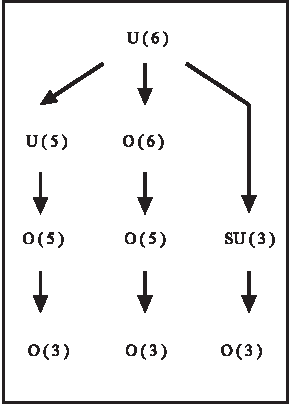
\includegraphics[scale=.65]{figure}
%
% If no graphics program available, insert a blank space i.e. use
%\picplace{5cm}{2cm} % Give the correct figure height and width in cm
%
\caption{If the width of the figure is less than 7.8 cm use the \texttt{sidecapion} command to flush the caption on the left side of the page. If the figure is positioned at the top of the page, align the sidecaption with the top of the figure -- to achieve this you simply need to use the optional argument \texttt{[t]} with the \texttt{sidecaption} command}
\label{fig:1}       % Give a unique label
\end{figure}


\paragraph{Paragraph Heading} %
Instead of simply listing headings of different levels we recommend to
let every heading be followed by at least a short passage of text.
Further on please use the \LaTeX\ automatism for all your
cross-references and citations as has already been described in
Sect.~\ref{sec:2}.

Please note that the first line of text that follows a heading is not indented, whereas the first lines of all subsequent paragraphs are.

For typesetting numbered lists we recommend to use the \verb|enumerate| environment -- it will automatically render Springer's preferred layout.

\begin{enumerate}
\item{Livelihood and survival mobility are oftentimes coutcomes of uneven socioeconomic development.}
\begin{enumerate}
\item{Livelihood and survival mobility are oftentimes coutcomes of uneven socioeconomic development.}
\item{Livelihood and survival mobility are oftentimes coutcomes of uneven socioeconomic development.}
\end{enumerate}
\item{Livelihood and survival mobility are oftentimes coutcomes of uneven socioeconomic development.}
\end{enumerate}


\subparagraph{Subparagraph Heading} In order to avoid simply listing headings of different levels we recommend to let every heading be followed by at least a short passage of text. Use the \LaTeX\ automatism for all your cross-references and citations as has already been described in Sect.~\ref{sec:2}, see also Fig.~\ref{fig:2}.

For unnumbered list we recommend to use the \verb|itemize| environment -- it will automatically render Springer's preferred layout.

\begin{itemize}
\item{Livelihood and survival mobility are oftentimes coutcomes of uneven socioeconomic development, cf. Table~\ref{tab:1}.}
\begin{itemize}
\item{Livelihood and survival mobility are oftentimes coutcomes of uneven socioeconomic development.}
\item{Livelihood and survival mobility are oftentimes coutcomes of uneven socioeconomic development.}
\end{itemize}
\item{Livelihood and survival mobility are oftentimes coutcomes of uneven socioeconomic development.}
\end{itemize}

\begin{figure}[t] %[t] sets the image at the top of the page; t = top, b = bottom, h = here%
\sidecaption[t]
% Use the relevant command for your figure-insertion program
% to insert the figure file.
% For example, with the option graphics use
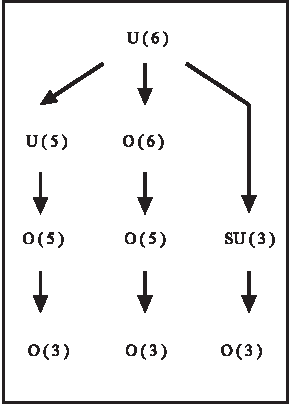
\includegraphics[scale=.65]{figure}
%
% If no graphics program available, insert a blank space i.e. use
%\picplace{5cm}{2cm} % Give the correct figure height and width in cm
%
%\caption{Please write your figure caption here}
\caption{If the width of the figure is less than 7.8 cm use the \texttt{sidecapion} command to flush the caption on the left side of the page. If the figure is positioned at the top of the page, align the sidecaption with the top of the figure -- to achieve this you simply need to use the optional argument \texttt{[t]} with the \texttt{sidecaption} command}
\label{fig:2}       % Give a unique label
\end{figure}

% Use the \index{} command to code your index words
% Make sure to inlcude the indexed word inside and outside of the brackets if you want the text to show up in your paragraph:
% e.g. This book is about \index{genetic programming}genetic programming. 
% If the text is not entered outside the brackets it will appear as: This book is about .
%
% For tables use
%
\begin{table}
\caption{Please write your table caption here}
\label{tab:1}       % Give a unique label
%
% Follow this input for your own table layout
%
\begin{tabular}{p{2cm}p{2.4cm}p{2cm}p{4.9cm}}
\hline\noalign{\smallskip}
Classes & Subclass & Length & Action Mechanism  \\
\noalign{\smallskip}\svhline\noalign{\smallskip}
Translation & mRNA$^a$  & 22 (19--25) & Translation repression, mRNA cleavage\\
Translation & mRNA cleavage & 21 & mRNA cleavage\\
Translation & mRNA  & 21--22 & mRNA cleavage\\
Translation & mRNA  & 24--26 & Histone and DNA Modification\\
\noalign{\smallskip}\hline\noalign{\smallskip}
\end{tabular}
$^a$ Table foot note (with superscript)
\end{table}
%
\section{Section Heading}
\label{sec:3}
% Always give a unique label
% and use \ref{<label>} for cross-references
% and \cite{<label>} for bibliographic references
Instead of simply listing headings of different levels we recommend to
let every heading be followed by at least a short passage of text.
Further on please use the \LaTeX\ automatism for all your
cross-references and citations as has already been described in
Sect.~\ref{sec:2}.

Please note that the first line of text that follows a heading is not indented, whereas the first lines of all subsequent paragraphs are.

If you want to list definitions or the like we recommend to use the Springer-enhanced \verb|description| environment -- it will automatically render Springer's preferred layout.

\begin{description}[Type 1]
\item[Type 1]{That addresses central themes pertainng to migration, health, and disease. In Sect.~\ref{sec:1}, Wilson discusses the role of human migration in infectious disease distributions and patterns.}
\item[Type 2]{That addresses central themes pertainng to migration, health, and disease. In Sect.~\ref{subsec:2}, Wilson discusses the role of human migration in infectious disease distributions and patterns.}
\end{description}

\subsection{Subsection Heading} %
In order to avoid simply listing headings of different levels we recommend to let every heading be followed by at least a short passage of text. Use the \LaTeX\ automatism for all your cross-references and citations citations as has already been described in Sect.~\ref{sec:2}.

Please note that the first line of text that follows a heading is not indented, whereas the first lines of all subsequent paragraphs are.

\begin{svgraybox}
If you want to emphasize complete paragraphs of texts we recommend to use the newly defined Springer class option \verb|graybox| and the newly defined environment \verb|svgraybox|. This will produce a 15 percent screened box 'behind' your text.

If you want to emphasize complete paragraphs of texts we recommend to use the newly defined Springer class option and environment \verb|svgraybox|. This will produce a 15 percent screened box 'behind' your text.
\end{svgraybox}


\subsubsection{Subsubsection Heading}
Instead of simply listing headings of different levels we recommend to
let every heading be followed by at least a short passage of text.
Further on please use the \LaTeX\ automatism for all your
cross-references and citations as has already been described in
Sect.~\ref{sec:2}.

Please note that the first line of text that follows a heading is not indented, whereas the first lines of all subsequent paragraphs are.

\begin{theorem}
Theorem text goes here.
\end{theorem}
%
% or
%
\begin{definition}
Definition text goes here.
\end{definition}

\begin{proof}
%\smartqed
Proof text goes here.
\qed
\end{proof}

\paragraph{Paragraph Heading} %
Instead of simply listing headings of different levels we recommend to
let every heading be followed by at least a short passage of text.
Further on please use the \LaTeX\ automatism for all your
cross-references and citations as has already been described in
Sect.~\ref{sec:2}.

Note that the first line of text that follows a heading is not indented, whereas the first lines of all subsequent paragraphs are.
%
% For built-in environments use
%
\begin{theorem}
Theorem text goes here.
\end{theorem}
%
\begin{definition}
Definition text goes here.
\end{definition}
%
\begin{proof}
\smartqed
Proof text goes here.
\qed
\end{proof}
%
\begin{acknowledgement}
If you want to include acknowledgments of assistance and the like at the end of an individual chapter please use the \verb|acknowledgement| environment -- it will automatically render Springer's preferred layout.
\end{acknowledgement}

\bibliographystyle{spbasic}
\bibliography{gp-bibliography,chapter}
